% Autor: Tony Pham xphamt00@stud.fit.vutbr.cz

\documentclass[12pt, letterpaper]{article}

\usepackage{pdfpages}
\usepackage{rotating}
\usepackage[czech]{babel}
\usepackage[utf8]{inputenc}
\usepackage[a4paper, total={6in, 8in}]{geometry}
\usepackage{graphicx} 

\begin{document}

	%%%%%%%%%%%%%%%%%%%%%%%%%%%%% Titulní stránka %%%%%%%%%%%%%%%%%%%%%%%%%%%%%%%%
	\begin{titlepage}
		\begin{center}
			\includegraphics[width=0.80\linewidth]{logo_cz.png} \\

			\vspace{\stretch{0.320}}

			\Huge{Projektová dokumentace} \\
			\LARGE{\textbf{Implementace překladače jazyka IFJ21}} \\
			\Large{Tým 047, Varianta I}
			\vspace{\stretch{0.600}}
		

			\Large
			\begin{tabular}{l l l}
			    Členové týmu: \\\\
				\textbf{Tomáš Bártů} & \textbf{(xbartu11)} & \quad 25\,\% \\
				Šimon Vacek  & (xvacek10) & \quad 25\,\% \\
				Vít Janeček  & (xjanec30) & \quad 25\,\% \\
				Tony Pham  & (xphamt00) & \quad 25\,\% \\\\\\
			\end{tabular}
		\end{center}
			{\Large \today}
		\hfill
	\end{titlepage}

	%%%%%%%%%%%%%%%%%%%%%%%%%%%%%%%% Obsah %%%%%%%%%%%%%%%%%%%%%%%%%%%%%%%%
	\pagenumbering{arabic}
	\setcounter{page}{1}
	\tableofcontents
	\clearpage
	
	%%%%%%%%%%%%%%%%%%%%%%%%%%%%% Řešení projektu %%%%%%%%%%%%%%%%%%%%%%%%%%%%%%%%
	\section{Řešení projektu}
	
	\subsection{Lexikální analýza}
    \large
    Jádro lexikální analýzy tvoří funkce \textbf{\textit{get\_token}}, která je implementována jako konečný automat. Vstupem jsou 2 parametry: struktura token a zdrojový kód jazyka ifj21. Po průchodu funkcí se do struktury token uloží \textbf{\textit{ID}} [typ tokenu: řetězec, klíčové slovo, číslo, EOL, EOF,…] a \textbf{\textit{VALUE}} [value může být typu: string, integer, keyword, double]). Funkce čte soubor znak po znaku na jehož základě rozhoduje do jakého stavu má jít využitím switche.\\\\

	\subsection{Syntaktická a sémantická analýza}
    \large
    Syntaktickou analýzu shora dolů jsme implementovali rekurzivně a nachází se v \textbf{\textit{parser.c}} a analýzu zdola nahoru precedenčně v \textbf{\textit{expression.c}}. Vstupem jsou tokeny generované scannerem.
    \\\\
    Pro kontrolu syntaxe výrazů jsme implementovali zásobík na terminály a neterminály v souboru   \textbf{\textit{term\_stack.c}}
    \\\\
    Sématická analýza stejně jako syntaktická je implementována v \textbf{\textit{parser.c}} a \textbf{\textit{expression.c}}.
    \\\\
    \newpage
    \textbf{\textit{Tabulka symbolů}} je implementovaná jednosměrně vázaným seznamem, do kterého lze přidávat rámce pouze na vrchol. Položka (rámec) v seznamu odpovídá jednomu bloku programu. Tento rámec má ukazatel na vrchol binárního vyhledávacího stromu, ve kterém už jsou identifikátry proměnných a funkcí.
    Struktura tabulky obsahuje ukazatel na globální rámec (\textbf{\textit{GlobalElement}}) s identifikátory funkcí a nejvyšší rámec (\textbf{\textit{TopLocalElement}}) s identifikátory proměnných tohoto rámce. Nejvyšší rámec dál ukazuje na předchozí rámce, které překryl.
    \\
     Uzel stromu s identifikátorem obsahuje data k němu se vztahující, tzn. např. datový typ u proměnné a seznam s parametry a návratovými hodnotami u funkce.\\\\
     Pro zjednodušení jsme se rozhodli neimplementovat vícenásobné přiřazení hodnot do proměnných. Rovněž neimplementujeme funkce s více návratovými hodnotami. \\
     Tabulka symbolů je k nalezení v souboru \textbf{\textit{symtable.c}} .
    
	\subsection{Generování cílového kódu}
	Rozhodli jsme se generovat kód bez optimalizací a to tak, že tiskneme přímo instrukce na standardní výstup.\\\\
    Výpis kódu vestavěných funkcí (reads, readi, readn, write, tointeger, substr, ord, chr) je v \textbf{\textit{buildIn.c}} . Dále jsme vytvořili pomocné funkce pro výpis instrukcí, které se často opakují a nachází se v \textbf{\textit{generate\_code.c}}.\\\\
    \\
    \newpage
    Samotné generování ifjcode21 a volání výše zmíněných funkcí je umístěné v \textbf{\textit{parser.c}} a \textbf{\textit{expression.c}}. Za zmínku stojí vyřešení stínění tím, že kopírujeme proměnné z nižšího rámce datového zásobníku do následujícího rámce. Pokud se hodnota dané proměnné změní, propaguje se změno do nižšího rámce. \\\\
    Na generování kódu pracovali všichni členové týmu a proto jsme zavedli konvence pro názvy návěští a proměnných. 
	%%%%%%%%%%%%%%%%%%%%%%%%%%%%%%%% Práce v týmu %%%%%%%%%%%%%%%%%%%%%%%%%%%%%%%%
	\section{Práce v~týmu}

	\subsection{Způsob práce v~týmu}
    
    \large
    Práci v týmu jsme pojali tak, že členové týmu si rozdělili úkoly na právě zpracovávané části tzn. nedělali jsme moduly. Na projektu jsme začali pracovat v půlce října.
    
	\subsection{Verzovací systém}
    
    \large
    Pro správu našich souborů jsme zvolili verzovací systém Git, který jsme hostovali na platformě GitHub. Zvolili jsme přístup pull-requestů na repozitář vedoucího týmu.
    
	\subsection{Komunikace}
	\large
	Jako komunikační prostředky jsme zvolili discord a messenger, kde jsme konzultovali aktuální témata k projektu. Později jsme se začali scházet ve školních prostorách, abychom mohli aktivněji řešit aktuální problémy. 

	\subsection{Rozdělení práce mezi členy týmu}
	\Large 
	\textbf{Tomáš Bártů:}\\\
	Návrh automatu, Korekce, Syntaktická analýza zdola nahoru, Sématická analýza, Abstraktí datové struktury, Debug, Generování kódu \\
	\\
	Šimon Vacek:\\
	Testy, LL gramatika, Syntaktická analýza shora dolu, Sématická analýza, Debug, Generování kódu\\
	\\\\
	Vít Janeček:\\
	Lex. analýza, Abstraktí datové struktury včetně tabulky symbolů, Debug, Generování kódu\\
	\\
	Tony Pham:\\
	Lex. analýza, Dokumentace, Oprava leaků, Debug, Generování kódu\\
	\newpage
	%%%%%%%%%%%%%%%%%%%%%%%%%%%%%%% Problémy při vývoji %%%%%%%%%%%%%%%%%%%%%%%%%%
	\section{Problémy při vývoji}
	\large
    Během implementace scanneru jsme v lexikální analýze museli řešit hned několik problému např.: přeskočení čtení znaku u některých stavů (pomohla nám funkce \textbf{\textit{ungetc}}), chybný návrh automatu (museli jsme často přidávat / opravovat stavy).
	\\
	\\
	Během syntaktické analýzy shora dolů se také projevily naše chabé dovednosti plánování. Pravidla LL gramatiky byly upraveny téměř jedenáctkrát a to i 3 dny před odevzdáním.
	\\
	\\
	Podcenili jsme časovou náročnost projektu, sice jsme začali poněkud brzy a ze začátku šlo vše bez problému, ale po dokončení lexikální analýzy se vývoj projektu zabrzdil.
	\\
	\\
	Při příštím týmovém projektu bychom se více zaměřili na tvorbu testů.
	\\
	\\
	U sémantické analýzy jsme narazili na problém kontroly datových typů. Ten jsme vyřešili implementací zásobníků datových typů v souboru \textbf{\textit{type\_stack.c}}.
	\\
	\\
	Většinu paměti se nám podařilo uvolnit, ale problémem byla neuvolněná paměť ve struktuře
	Token.
	\\
	\\
	S většující se složitostí struktury bylo obtížnější správně uvolnit všechnu paměť.
	\newpage
	%%%%%%%%%%%%%%%%%%%%%%%%%%%%%% Použité zdroje %%%%%%%%%%%%%%%%%%%%%%%%%%%%%%%%
	\section{Použité nástroje, programy a literatura}

\begin{itemize}
\normalsize
  \item Prof. RNDr. Alexandr Meduna CSc. a Ing. Roman Lukáš Ph.D. - Formální jazyky a překladače, prezentace k přednáškám
  \item Ing. Bohuslav Křena Ph.D., Ing. Ivana Burgetová Ph.D. - Algoritmy, prezentace k přednáškám
  \item Ing. Zbyněk Křivka Ph.D. - Demonstrační cvičení IFJ, Implementace překladače IFJ21
  \item Prof. RNDr. Milan Češka, CSc.- Teoretická informatika, Učební texty
  \item Clion, https://www.jetbrains.com/clion/
  \item GitHub, https://github.com/paetricc/IFJ-Project
  \item Vim, https://www.vim.org
  \item QFSM, http://qfsm.sourceforge.net
  
\end{itemize}
	%%%%%%%%%%%%%%%%%%%%%%%%%%%% Diagram automatu %%%%%%%%%%%%%%%%%%%%%%%%%%%%%%%%
	\begin{sidewaysfigure}
        \section{Diagram automatu}
	        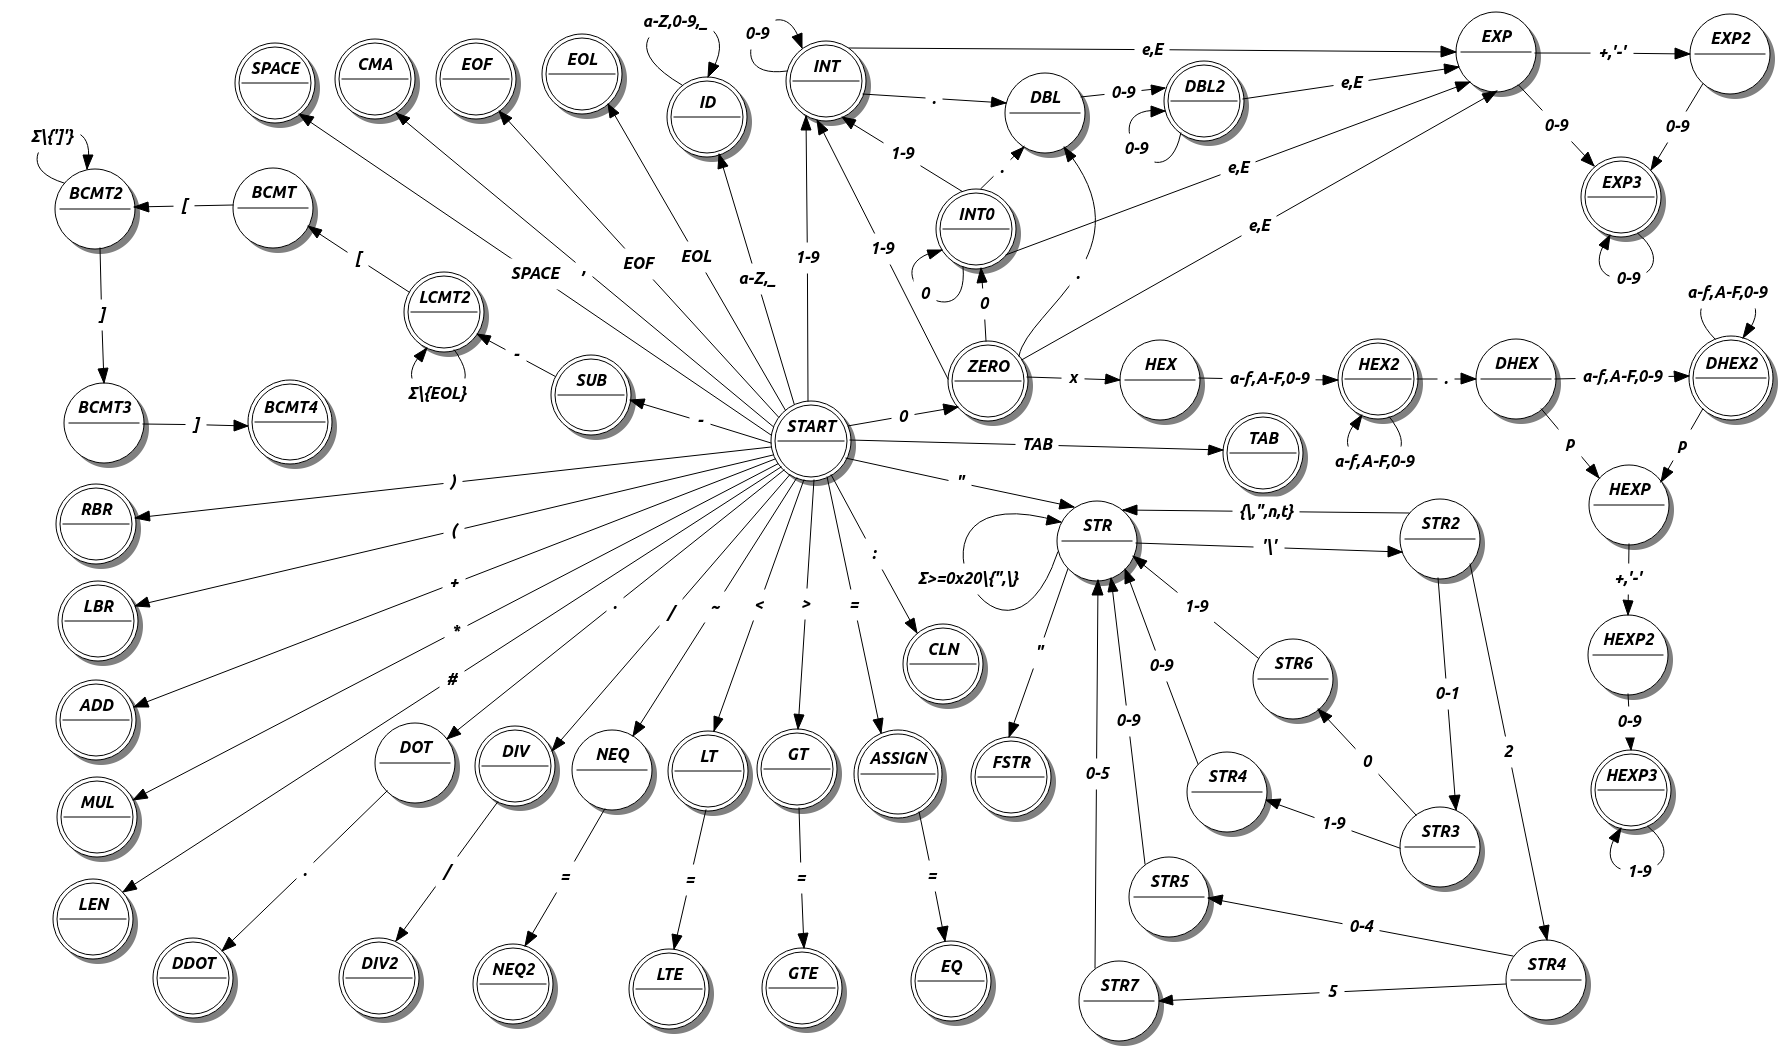
\includegraphics[width=\textwidth,height=\textheight,keepaspectratio]{LexAnalyzatorFSM.png}
    \end{sidewaysfigure}
    \newpage
    	%%%%%%%%%%%%%%%%%%%%%%%%%%%% Tabulka symbolů %%%%%%%%%%%%%%%%%%%%%%%%%%%%%%%%
	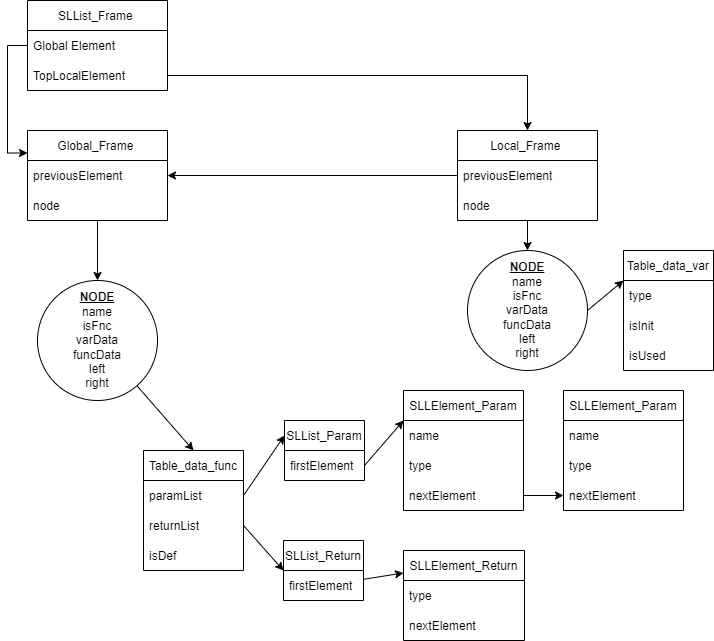
\includepdf[scale=0.75 ,pages=1,pagecommand=\section{Tabulka symbolů}]{Symtable.pdf}
    \newpage
	%%%%%%%%%%%%%%%%%%%%%%%%% Precedenční tabulka %%%%%%%%%%%%%%%%%%%%%%%%%%%%%%%%
	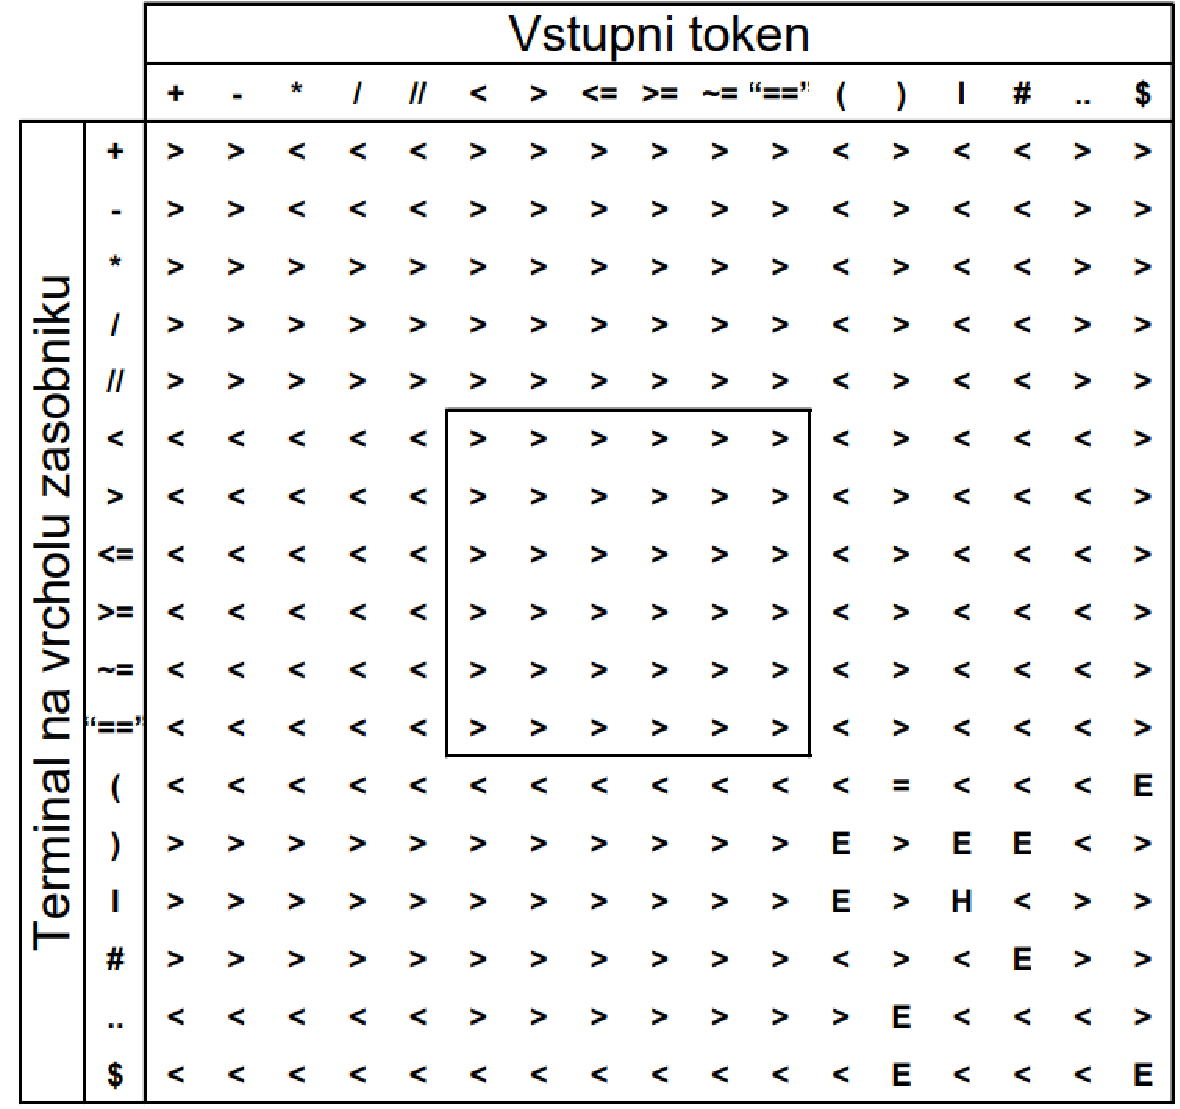
\includepdf[scale=0.83 ,pages=1,pagecommand=\section{Precedenční tabulka}]{precedenceTable.pdf}
 \newpage
 	%%%%%%%%%%%%%%%%%%%%%%%%% Gramatika pro výrazy %%%%%%%%%%%%%%%%%%%%%%%%%%%%%%%%
	\section{Gramatika pro výrazy}
	\begin{enumerate}
 \item EXP $\rightarrow$ i
 \item EXP $\rightarrow$ EXP + EXP
 \item EXP $\rightarrow$ EXP - EXP
 \item EXP $\rightarrow$ EXP * EXP
 \item EXP $\rightarrow$ EXP / EXP
 \item EXP $\rightarrow$ EXP // EXP
 \item EXP $\rightarrow$ EXP .. EXP
 \item EXP $\rightarrow$ (EXP)
 \item EXP $\rightarrow$ EXP $<$ EXP
 \item EXP $\rightarrow$ EXP $>$ EXP
 \item EXP $\rightarrow$ EXP $<$= EXP
 \item EXP $\rightarrow$ EXP $>$= EXP
 \item EXP $\rightarrow$ EXP $\sim$= EXP
 \item EXP $\rightarrow$ EXP == EXP
 \item EXP $\rightarrow$ $\#$EXP
 \end{enumerate}
 
    %%%%%%%%%%%%%%%%%%%%%%% Pravidla LL gramatiky %%%%%%%%%%%%%%%%%%%%%%%%%%%%%%%%
  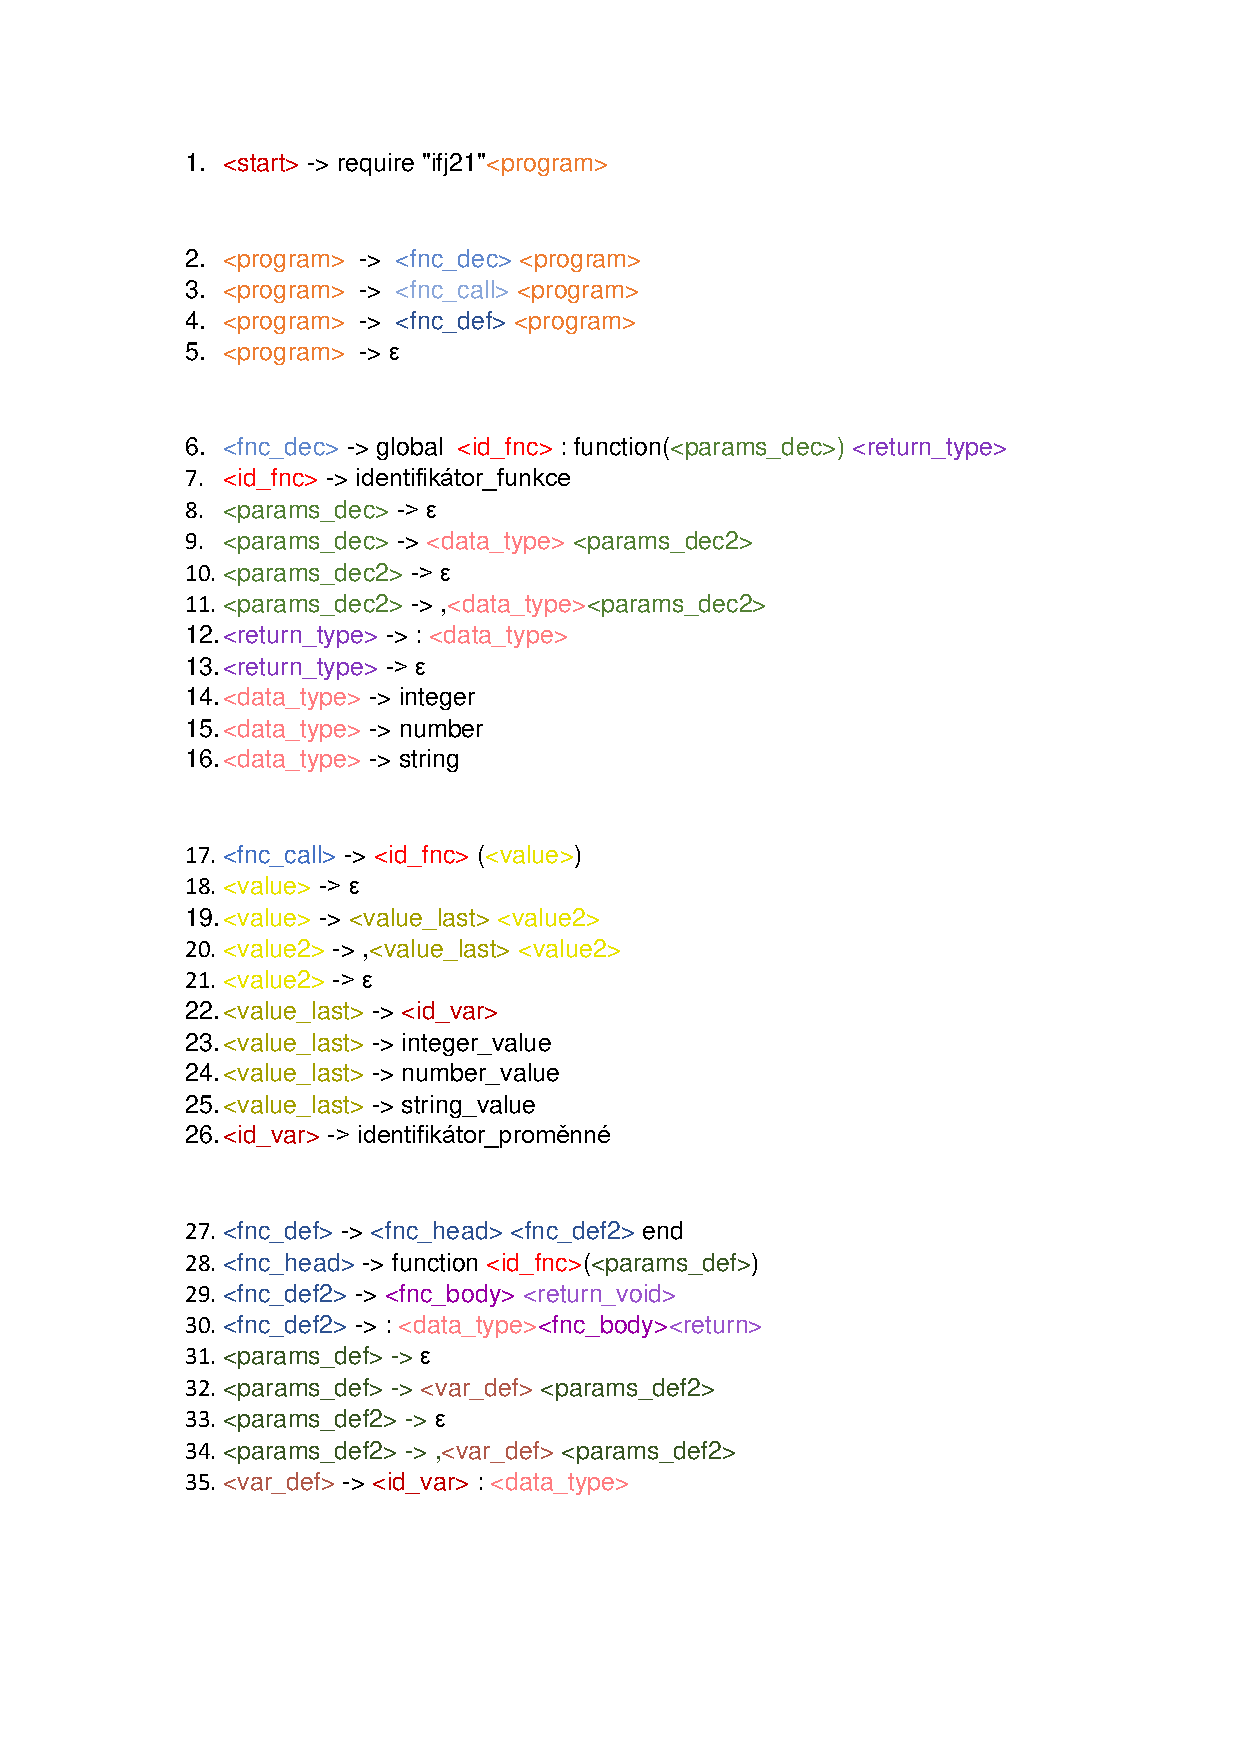
\includepdf[scale=0.83,pages=1,pagecommand=\section{Pravidla LL gramatiky}]{LLGramatika.pdf}
  \newpage
  \includepdf[scale=0.83,pages=2]{LLGramatika.pdf}

  %%%%%%%%%%%%%%%%%%%%%%%%%%%%%%%% LL tabulka %%%%%%%%%%%%%%%%%%%%%%%%%%%%%%
	\begin{sidewaysfigure}
        \section{LL tabulka}
	        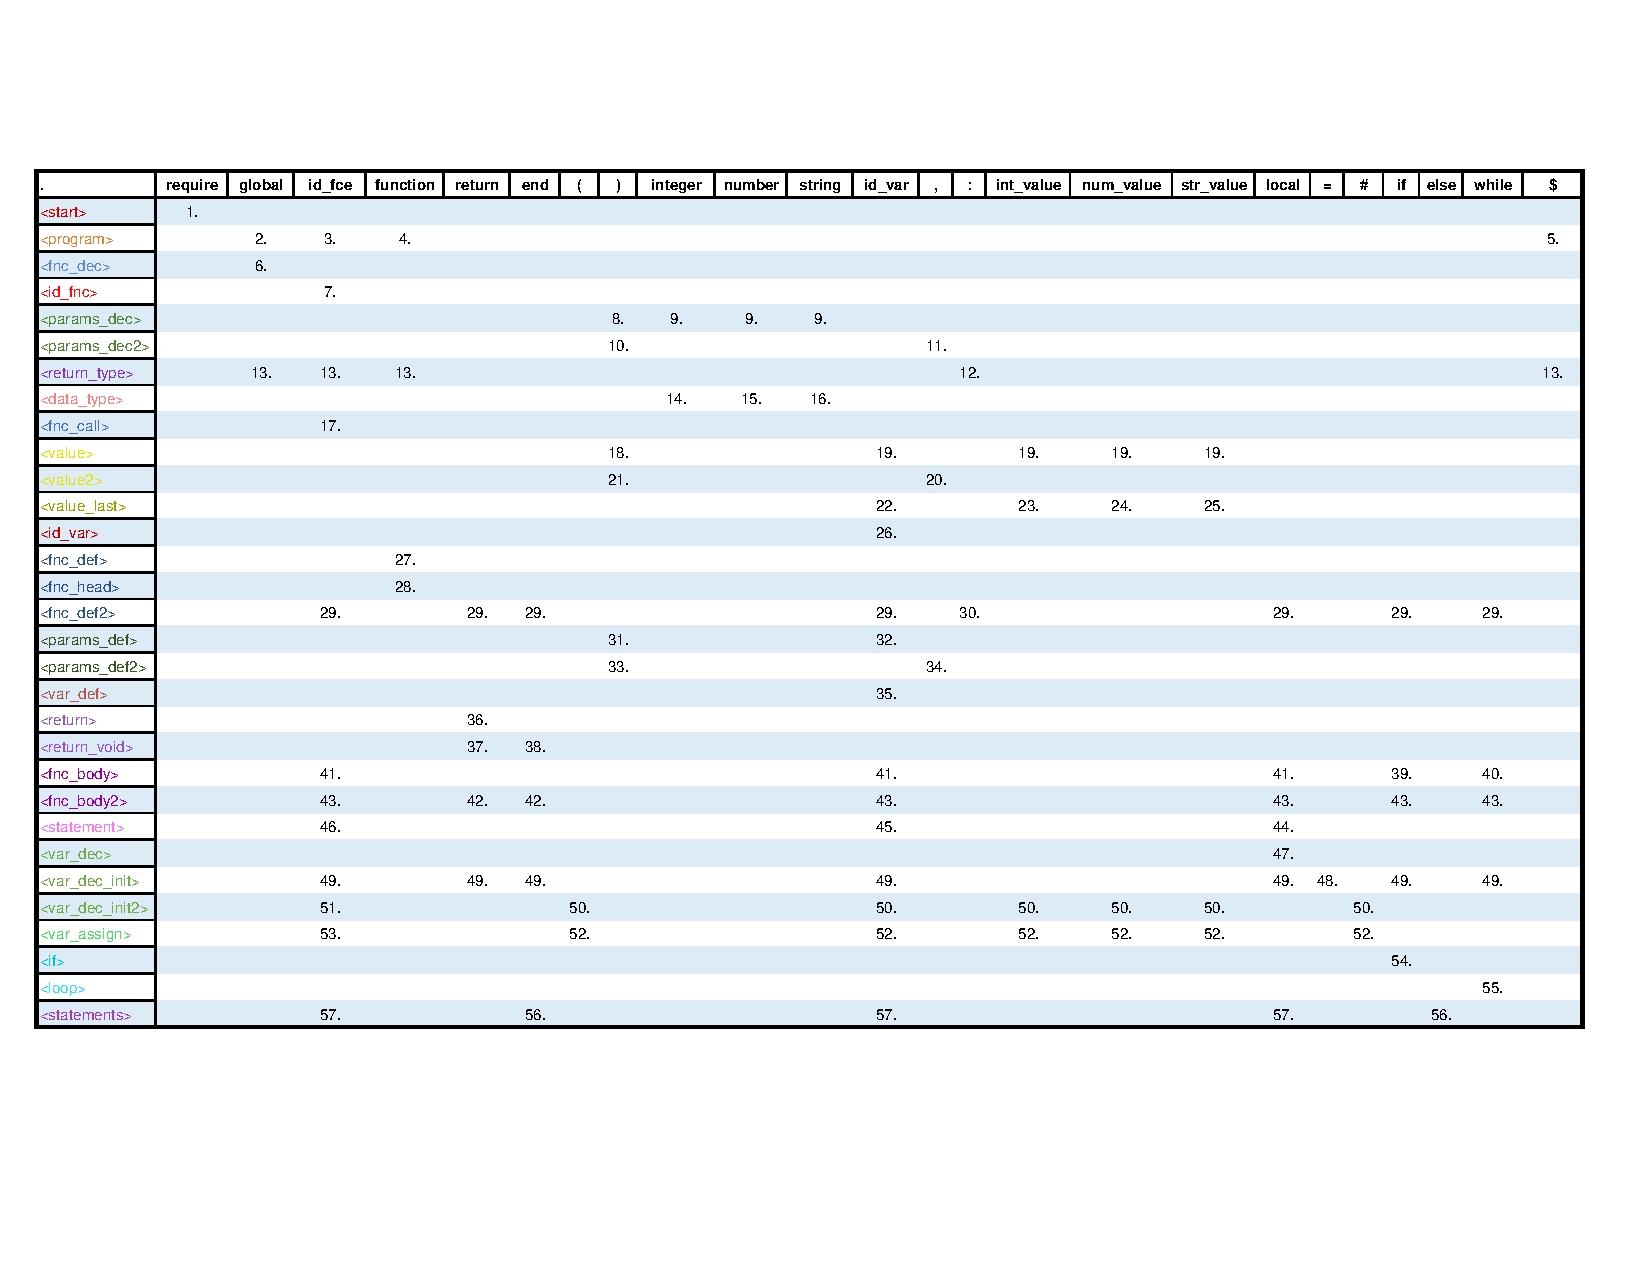
\includegraphics[width=\textwidth,height=\textheight,keepaspectratio]{LLTabulka.pdf}
    \end{sidewaysfigure}
    
\end{document}